\documentclass[11pt,a4paper]{article}
\usepackage[margin=22mm,headheight=16pt]{geometry}
\usepackage{fontspec,xeCJK}
\setmainfont{Times New Roman}
\setsansfont{Arial}
\setmonofont{Consolas}[Scale=0.88]
\setCJKmainfont{SimSun}[BoldFont=Microsoft YaHei]
\setCJKsansfont{Microsoft YaHei}
\setCJKmonofont{SimSun}
\usepackage{amsmath,amssymb,booktabs,tabularx,array,enumitem}
\usepackage[table]{xcolor}
\usepackage{fancyhdr,fvextra,hyperref,titlesec}
\usepackage{graphicx}
\definecolor{inkblue}{HTML}{234D66}
\definecolor{lightblue}{HTML}{EDF3F6}
\definecolor{muted}{HTML}{59636B}
\hypersetup{colorlinks=true,urlcolor=inkblue,linkcolor=inkblue,
 pdftitle={反馈驱动的语言模型与程序优化：两个小规模实证案例},pdfauthor={Research Contributors}}
\setlength{\parindent}{0pt}
\setlength{\parskip}{4pt}
\clubpenalty=10000
\widowpenalty=10000
\displaywidowpenalty=10000
\setlength{\emergencystretch}{1em}
\renewcommand{\baselinestretch}{1.16}
\renewcommand{\arraystretch}{1.18}
\setlist{nosep,leftmargin=1.6em,topsep=3pt}
\setcounter{secnumdepth}{2}
\titleformat{\section}{\Large\bfseries\sffamily\color{inkblue}}{\thesection}{0.6em}{}
\titleformat{\subsection}{\large\bfseries\sffamily\color{inkblue}}{\thesubsection}{0.6em}{}
\titlespacing*{\section}{0pt}{10pt}{6pt}
\pagestyle{fancy}
\fancyhf{}
\fancyhead[L]{\small\sffamily\color{muted} 反馈驱动优化研究}
\fancyhead[R]{}
\fancyfoot[C]{\small\color{muted}\thepage}
\renewcommand{\headrulewidth}{0.3pt}
\newcolumntype{Y}{>{\raggedright\arraybackslash}X}
\newcolumntype{P}[1]{>{\raggedright\arraybackslash}p{#1}}
\newcommand{\key}[1]{\textbf{#1}}
\newcommand{\smallheading}[1]{\par\medskip{\large\bfseries\color{inkblue}#1}\par\nobreak\smallskip\nobreak}
\newcommand{\code}[1]{\texttt{#1}}
\newcommand{\tablehead}{\rowcolor{lightblue}}
\providecommand{\TrainableCount}{Pending}
\providecommand{\TotalCount}{Pending}
\providecommand{\BaseCount}{Pending}
\providecommand{\TrainableRatio}{Pending}
\providecommand{\ReplacedCount}{Pending}


\newcommand{\figcaption}[2]{\refstepcounter{figure}\label{#1}\par\smallskip
 {\small\color{muted}图~\thefigure：#2\par}\medskip}
\newcommand{\tablecaption}[2]{\refstepcounter{table}\label{#1}\par\smallskip
 {\small\color{muted}表~\thetable：#2\par}\smallskip}



\renewcommand{\TrainableCount}{4,399,104}
\renewcommand{\TotalCount}{498,431,872}
\renewcommand{\BaseCount}{494,032,768}
\renewcommand{\TrainableRatio}{0.8826\%}
\renewcommand{\ReplacedCount}{168}
% Measured constants from the successful A10 BF16 run.
\newcommand{\PPORolloutSteps}{32}
\newcommand{\PPONonzeroBTensors}{168}
\newcommand{\PPOBTensors}{168}
\newcommand{\PPOCriticNonzeroBTensors}{169}
\newcommand{\PPOCriticBTensors}{169}
\newcommand{\PPOBaselineCorrect}{117}
\newcommand{\PPOTrainedCorrect}{122}
\newcommand{\PPOValidationN}{128}
\newcommand{\PPOBaselineAccuracy}{91.40625\%}
\newcommand{\PPOTrainedAccuracy}{95.3125\%}
\newcommand{\PPODelta}{+3.90625}

\let\tabcaption\tablecaption
\begin{document}
\begin{center}
{\LARGE\bfseries\sffamily\color{inkblue} 反馈驱动的语言模型与程序优化\par}
\vspace{3mm}
{\large 两个小规模实证案例\par}
\vspace{2mm}
{\small 8 November 2026}
\end{center}
\section*{摘要}
本研究用两个小规模案例，考察可执行反馈怎样指导语言模型系统的优化，以及怎样验证优化是否真正发生。第一个案例实现 LoRA 低秩适配，并以固定版本 OpenRLHF 对 \path{Qwen/Qwen2.5-0.5B} 进行 PPO 算术任务训练。独立的功能检查覆盖参数冻结、数值等价与合并；随后在 NVIDIA A10 上，以 BF16 完成 512 道训练题、32 个采样批次、适配器保存及 Actor 重载。同一组 128 道开发验证题的首行整数答案正确数由 117 增至 122，变化为 3.90625 个百分点。第二个案例在 LLM4AD\_Next 平台用真实模型调用搜索 26 圆布局程序，保存了 5 次有效在线评估，最佳在线半径和为 2.62001380699489；导出程序的独立本地复现另得 2.6206092130170973。两个数值来自不同记录，分别保留。研究未进行多随机种子或超参数消融；在线搜索手动停止，也未证明全局最优。本文的主要产出是可检查的实现、实验结果及证据链，而不是通用推理能力或新优化算法的证明。

{\small\color{muted}\key{关键词：}低秩适配；PPO；程序搜索；外部评估；实验复核。中文说明与英文报告采用相同数据和结论，另补充必要的概念解释。}

\section{引言与研究问题}
语言模型系统可以在不同层面接受反馈。一种方式是调整模型参数，使以后生成某种回答的概率发生变化；另一种方式是保留模型本身，通过反复生成、执行和筛选代码，改变最终使用的程序。前者的优化对象是参数，后者的优化对象是程序。两者都需要把“看起来合理”与“经过执行验证”分开。

本研究围绕两个具体问题展开：
\begin{enumerate}
\item 在小型算术任务上，能否完成从 LoRA 实现、PPO 训练，到保存、重载和同条件评估的可检查流程？实际任务分数怎样变化？
\item 在固定的几何约束和有限搜索记录中，大模型引导的程序搜索能否产生有效候选？在线分数和独立复现分别支持什么结论？
\end{enumerate}
这两个案例的任务、指标和预算不同，因此不是 LoRA-PPO 与程序搜索之间的优劣对比。共同考察的是反馈怎样进入系统、结果怎样测量，以及哪些额外检查能防止把过程日志误当成最终成功。

\begin{minipage}{\linewidth}
\par\noindent\begin{minipage}{\linewidth}
\begin{center}
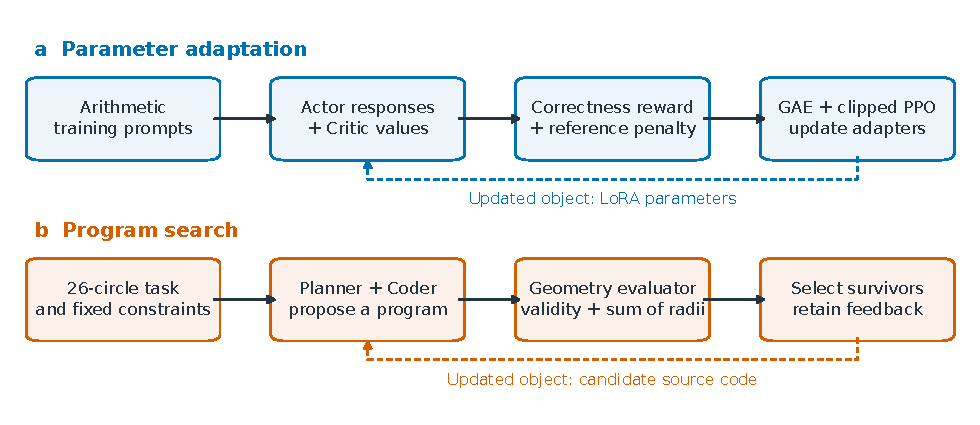
\includegraphics[width=166mm]{../../figures/feedback_mechanisms.pdf}
\end{center}
\figcaption{fig:feedback-zh}{两种反馈驱动优化的机制示意。参数适应改变 LoRA 参数，程序搜索改变候选代码；图用于解释研究设计，不是实验分数、平台截图或新增算法的证明。}
\end{minipage}\par

\end{minipage}

实施过程中，除了记录成功运行，也保留了早期模型保存失败、下载中断、运行保护和在线无效候选。正文先说明方法和设计，再报告已核实的结果；附录保留实现说明、历史保存失败、运行范围及复现索引。

\section{方法与实验设计}
\subsection{低秩参数适应：把数学落实为可验证的实现}
模型参数是计算输出时使用的数字。前向计算得到输出，反向传播计算损失对参数的梯度，优化器才真正修改参数。LoRA 是参数高效微调的一种方式：冻结原来的大权重，只训练附加的小矩阵。\cite{lora,lorasurvey}

对列向量输入 $\boldsymbol{x}\in\mathbb{R}^{d_{\mathrm{in}}}$，原线性层为 $W\boldsymbol{x}+\boldsymbol{b}$。LoRA 引入
\[
W\in\mathbb R^{d_{\mathrm{out}}\times d_{\mathrm{in}}},\qquad
A\in\mathbb R^{r\times d_{\mathrm{in}}},\qquad
B\in\mathbb R^{d_{\mathrm{out}}\times r}.
\]
\begin{align}
\Delta W&=\frac{\alpha}{r}BA,\quad r>0,\label{eq:lora-zh}\\
\boldsymbol{y}&=W\boldsymbol{x}+\boldsymbol{b}
+\frac{\alpha}{r}BA\boldsymbol{x}.\label{eq:lora-forward-zh}
\end{align}
$r$ 是中间空间的宽度，也是修正矩阵秩的上界；$\alpha/r$ 控制新增路径的幅度。$A$ 先把输入映射到较小空间，$B$ 再映射回输出维度。训练时更新 $A,B$，原来的 $W,\boldsymbol b$ 保持冻结。

\begin{minipage}{\linewidth}
\par\noindent\begin{minipage}{\linewidth}
\begin{center}
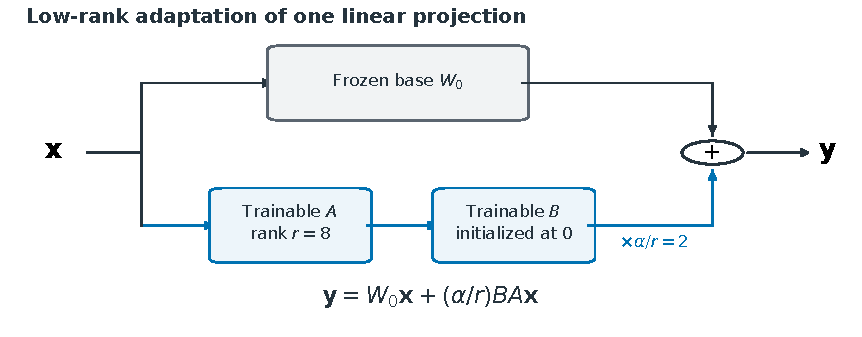
\includegraphics[width=146mm]{../../figures/lora_mechanism.pdf}
\end{center}
\figcaption{fig:lora-zh}{LoRA 原路径与低秩修正路径。两条路径的输出相加；示意图用于解释式~\eqref{eq:lora-forward-zh}，不表示已经完成训练。}
\end{minipage}\par

\end{minipage}

忽略偏置，原权重包含 $d_{\mathrm{in}}d_{\mathrm{out}}$ 个参数，LoRA 新增 $r(d_{\mathrm{in}}+d_{\mathrm{out}})$ 个。若两个维度均为 1024、$r=8$，原权重为 1,048,576 个参数，新增为 16,384 个。但完整模型仍要保存冻结权重并参与计算，所以可训练参数比例不等于显存节省比例。

实现采用随机初始化 $A$、零初始化 $B$，使初始 $BA=0$，保持原层输出。推理时可合并 $W\leftarrow W+\Delta W$；之后必须关闭新增路径，避免重复相加。PyTorch 的批量输入按行存放，关闭 dropout 时对应
\[
Y=XW^{\mathsf T}+\boldsymbol{1}_m\boldsymbol b^{\mathsf T}
 +\frac{\alpha}{r}XA^{\mathsf T}B^{\mathsf T}.
\]
六处具体实现、$r=0$ 的边界处理和手工实现输出保存在附录~\ref{app:implementation-zh}。

\subsection{学习率与批大小：设计依据，而非已完成的消融实验}
学习率决定每次参数更新的尺度。最简单的梯度下降写成
\begin{equation}
\boldsymbol{\theta}_{t+1}
=\boldsymbol{\theta}_t-\eta\nabla_{\boldsymbol{\theta}}\mathcal L(\boldsymbol{\theta}_t).
\label{eq:learning-rate-zh}
\end{equation}
这里 $\eta$ 是学习率，梯度给出损失对参数变化的敏感方向；实际 Adam 还利用历史梯度。学习率较小可能更温和，但在有限步数内进展较慢；较大可能加快初期变化，也可能越过合适区域或使优化不稳定。

批大小表示一次有效更新使用多少样本。若固定 1,024 条数据且不做梯度累积，批大小 8 对应 128 次更新，批大小 64 只有 16 次更新。因此比较批大小时，必须说明固定的是数据量、更新次数还是计算预算。较大批量通常降低梯度波动，却可能增加显存需求；较小批量节约单次显存，但梯度更有噪声，设备利用率也可能较低。文本长度同样会影响成本。

\textit{LoRA Without Regret} 在其研究设置中观察到：LoRA 合适的学习率约为全参数微调的十倍；一些大批量设置会扩大差距，单纯提高秩也未消除差距。\cite{lorablog} 这些是该文的经验结果，不是所有任务通用的规则。本研究据此理解学习率、秩、缩放和批量的相互影响，但只采用一个训练配置，没有实测学习率或批大小的优劣。

\subsection{PPO 与外部奖励}
LoRA 决定哪些参数可以更新；PPO 决定怎样根据奖励更新它们。实际训练使用 OpenRLHF 集成的 PEFT 适配器，手写 LoRA 层用于理解和功能验证；二者不是把同一个手写层直接替换进整个 PPO 框架。这里使用可执行的算术评分规则，没有收集人类偏好数据。

\par\noindent\begin{minipage}{\linewidth}
\tablecaption{tab:roles-zh}{训练中的四种角色及其区别。}
\begin{tabularx}{\linewidth}{@{}P{32mm}Y@{}}
\toprule
\tablehead \key{角色} & \key{作用}\\
\midrule
Actor：策略模型 & Qwen 加 LoRA，逐个 token 生成回答；token 是模型处理文字的基本单位。\\
Critic：价值模型 & 预测后续回报，帮助计算行为相对预期的优势。\\
Reference：固定参照 & 保留初始模型，用于约束策略偏离。\\
Reward：外部评分 & 本地 HTTP 服务核对首行整数，给出 0 或 1 的任务奖励。\\
\bottomrule
\end{tabularx}
\end{minipage}\par


PPO 比较当前策略和生成这一批样本时的旧策略，裁剪目标为\cite{ppo}
\begin{align}
\rho_t(\boldsymbol{\theta})
&=\frac{\pi_{\boldsymbol{\theta}}(a_t\mid s_t)}
{\pi_{\mathrm{old}}(a_t\mid s_t)},\\
J_{\mathrm{clip}}(\boldsymbol{\theta})
&=\mathbb E_t\!\left[
\min\!\left(\rho_t\widehat A_t,\,
\operatorname{clip}(\rho_t,1-\epsilon,1+\epsilon)\widehat A_t\right)\right].
\label{eq:ppo-zh}
\end{align}
$s_t$ 是当前上下文，$a_t$ 是生成的 token，$\widehat A_t$ 是优势估计。概率比值 $\rho_t$ 与 LoRA 的秩 $r$ 不是同一个量。例如概率从 0.2 增至 0.3，概率比值为 1.5；当 $\epsilon=0.2$，裁剪后的比值为 1.2。裁剪限制目标收益，却不严格保证策略距离一定小于某个值。

本实验使用 Critic 和 GAE。忽略终止位置的掩码时，可按下面两步理解优势：
\[
\delta_t=\widetilde r_t+\gamma V(s_{t+1})-V(s_t),\qquad
\widehat A_t=\sum_{\ell=0}^{T-t-1}(\gamma\lambda)^\ell\delta_{t+\ell}.
\]
其中 $\widetilde r_t$ 是包含相对 Reference 约束的实际奖励；优势衡量的是“获得的反馈比原先预计好多少”。PPO 的旧策略只对应当前采样批次，Reference 则固定为初始模型，二者不能混用。初始 KL 系数为 $\beta=0.01$。

\subsection{算术任务与配对验证协议}
\path{policy_adaptation/prepare_ppo_data.py} 以种子 1234，从 $0\le a\le b<50$ 的加法数对中产生 512 道训练题和 128 道开发验证题。两组互不交叠，交换加数后的等价题也不会跨组；提示里的两道示例排除在两组之外。每行 JSONL 保存提示、标准答案和加数。实际分词检查中最长提示为 53 tokens，低于 192 的上限。

评分器只检查新增回答的第一行：允许水平空格和正负号，但整行必须是与答案相同的整数。首行 \code{7} 可以答对 $3+4$；\code{7 because...} 不符合格式。后续行不能挽救错误首行，也不作为简洁性指标。HTTP 请求包含完整提示和回答，评分器先核对并移除提示前缀，避免把示例答案误算成生成结果。

早期输出曾用于调整评分协议，因此这 128 题是\key{开发验证集}，不是完全未参与设计的最终测试集。11 月 8 日的比较在规则确定后重新测量：前后采用同一题序、BF16、贪心解码、32 个新 token 上限和同一评分函数。旧 FP32 T4 的 118/128 不进入此次差值。

\par\noindent\begin{minipage}{\linewidth}
\tablecaption{tab:ppo-design-zh}{实际 A10 实验的固定设置。}
\begin{tabularx}{\linewidth}{@{}P{59mm}Y@{}}
\toprule
\tablehead \key{项目} & \key{设置}\\
\midrule
基础模型 & \path{Qwen/Qwen2.5-0.5B}，固定修订；不是 Instruct 版。\\
LoRA & $r=8$，$\alpha=16$，dropout 为 0。\\
Actor / Critic 学习率 & $10^{-5}$ / $5\times10^{-5}$。\\
采样 / 有效训练批量 & 16 / 8；两个 micro batch 均为 1。\\
PPO 设置 & GAE，$\gamma=1$，$\lambda=0.95$，$\epsilon=0.2$，初始 $\beta=0.01$。\\
长度与预算 & 输入上限 192、输出上限 32 tokens；512 题，1 episode、1 epoch。\\
计算环境 & 单 NVIDIA A10、BF16、ZeRO-2、梯度检查点。\\
软件 & Python 3.10；PyTorch 2.5.1+cu124；Transformers 4.48.3；PEFT 0.14.0；DeepSpeed 0.16.3。\\
\bottomrule
\end{tabularx}
\end{minipage}\par


micro batch 是单次处理量，有效批量还包含梯度累积；rollout batch 则是一次生成回答的数量。梯度检查点通过重算中间结果节省显存，不等于保存模型文件。OpenRLHF 固定为 v0.6.0、提交 \code{bfa85f6fa8cd6214707f93883fac5d08334f4f06}。\cite{openrlhf} 基础模型固定修订为\newline\code{060db6499f32faf8b98477b0a26969ef7d8b9987}。\cite{qwen} ModelScope 只作为下载传输来源，其 \code{master} 标识不冒充固定模型修订。模型七个运行文件与原始清单逐项核对，权重未替换。流程先独立运行 16 题，检查保存和 Actor 重载；通过后从原始基座重新训练完整 512 题，不从短实验的适配器接着训练。

\subsection{大模型引导的程序搜索}
LLM4AD\_Next，也称 OpenLoopX，通过“提出方案、生成代码、执行评估、选择候选”的循环搜索程序。\cite{llm4ad,architecture} 这里变化的是代码，不是大模型权重。模型可承担多个角色；五个组件并不意味着训练了五个独立模型。

\begin{minipage}{\linewidth}
\par\noindent\begin{minipage}{\linewidth}
\begin{center}
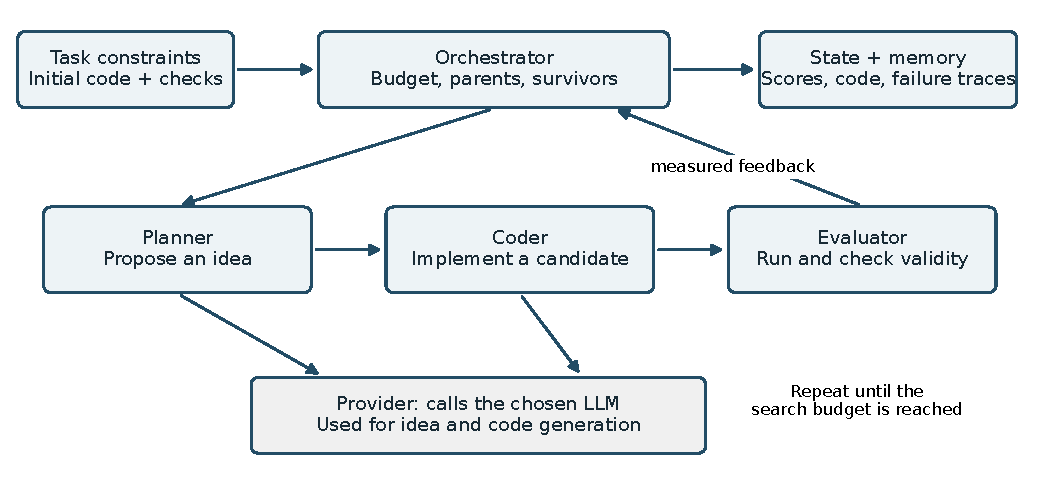
\includegraphics[width=\linewidth]{../../program_search/figures/framework.pdf}
\end{center}
\figcaption{fig:framework-zh}{依据官方架构和数据流资料绘制的解释性框架图。Provider 连接模型，Planner 提出修改，Coder 生成代码，Evaluator 执行检查，Orchestrator 管理选择、迁移与停止。\cite{architecture,dataflow} 保存配置和实际停止范围另见附录~\ref{app:online-zh}。}
\end{minipage}\par

\end{minipage}

一次迭代先固定任务接口、约束和评估器，再在允许修改的代码区域产生候选。评估器执行它，记录分数或失败；搜索机制据此选择后续父程序。Island GA 让多个群体分开搜索并偶尔交换候选，有助于保留不同方向，但频繁迁移也可能让它们趋同。记忆和反思能复用经验，却需要额外检索和可靠性控制。\cite{islands,memory}

本研究选择单位正方形内 26 个圆的布局任务。\cite{benchmark,circle} 对圆心 $\boldsymbol c_i=(x_i,y_i)$ 和半径 $r_i$，
\begin{align}
\max_{\{\boldsymbol c_i,r_i\}_{i=1}^{26}}\quad
&S=\sum_{i=1}^{26}r_i, \label{eq:circle-objective-zh}\\
\text{满足}\quad
&r_i\ge0,\quad r_i\le x_i\le1-r_i,\quad r_i\le y_i\le1-r_i,\\
&\|\boldsymbol c_i-\boldsymbol c_j\|_2\ge r_i+r_j,\quad i<j.
\end{align}
目标是\key{半径之和}，不是覆盖面积。评估还要求有限的 $(26,2)$ 圆心数组和 $(26,)$ 半径数组。只看图片是否紧密，不能替代几何检查。

在线实验使用真实 \code{deepseek-v4-flash} 调用、种子 42，保存预算为 2 个岛、每岛初始目标 2 个候选及 2 代演化，最多 2 个并发请求，Coder 输出上限为 32,768 tokens。2026 年 10 月 31 日修正版的记录覆盖初始化、第 1 代及第 2 代开始；最后导出后手动停止。本文统计实际完成的评估，不把保存预算写成已经全部执行的次数。



保存配置采用锦标赛父代选择、截断式保留，变异率为 0.3、交叉率为 0.5、精英比例为 0.2；迁移间隔为 1，拓扑为环形。Coder 温度为 0.7，保存的上下文上限为 8,192。评估器不重试。记忆提取被关闭，但运行日志仍出现评估轨迹嵌入，因此不能据此断言所有记忆操作均未发生。这些配置限定了实验解释范围，不能保证另一时点的托管服务产生相同程序。

\section{实验结果}
\subsection{LoRA 实现与功能验证}
手工实现在Qwen 基础模型上完成了注入、参数统计、前向计算和合并。实际替换 \ReplacedCount{} 个线性层，新增可训练参数为 \TrainableCount{}，含适配器的总参数为 \TotalCount{}，比例为 \TrainableRatio{}。这说明实现能够以较小的可训练参数集合工作，但该比例不代表实测显存节省。

九项测试覆盖初始等价、共享原权重、非零修正、合并等价及幂等、模块替换、非法配置、数据划分和真实奖励 HTTP 接口。其中小层测试实际执行了优化器更新，确认冻结参数不变。原 \code{main()} 本身没有优化器步骤，故其打印成功不能单独证明语言模型微调效果。完整输出与实现说明见附录~\ref{app:implementation-zh}。

\subsection{完整参数优化实验与同条件验证}
2026 年 11 月 8 日的 A10 BF16 实验完成 512 道训练题、\PPORolloutSteps{} 批采样，训练进程以退出码 0 结束；进度条显示训练循环约 12 分 02 秒，不含模型下载、安装、训练前后评估。独立的 16 题保存与 Actor 重载检查先通过，完整运行随后重新从原始基座开始。

Actor 的 \PPONonzeroBTensors{}/\PPOBTensors{} 个 LoRA B 张量、Critic 的 \PPOCriticNonzeroBTensors{}/\PPOCriticBTensors{} 个 B 张量非零；下载的全部适配器值和记录的标量均为有限数。与只看“开始运行”的日志相比，这些检查直接支持参数已更新并保存。

\par\noindent\begin{minipage}{\linewidth}
\tablecaption{tab:paired-zh}{同一组 128 道开发验证题的配对结果。}
\begin{tabularx}{\linewidth}{@{}Y P{38mm}P{38mm}@{}}
\toprule
\tablehead \key{指标} & \key{训练前} & \key{训练后}\\
\midrule
首行整数答案正确题数 & \PPOBaselineCorrect{}/\PPOValidationN & \PPOTrainedCorrect{}/\PPOValidationN\\
正确率 & \PPOBaselineAccuracy & \PPOTrainedAccuracy\\
相对基线的绝对变化 & --- & \PPODelta{} 个百分点\\
\bottomrule
\end{tabularx}
\end{minipage}\par


逐题复核发现：117 题前后均正确，5 题由错变对，6 题前后均错，没有由对变错的题。净增加 5 道正确答案与总体差值一致。两次评估使用相同 BF16 精度、贪心解码、生成长度和评分规则；图~\ref{fig:paired-zh} 保留每一道题，而不只展示两个汇总百分比。

\begin{minipage}{\linewidth}
\par\noindent\begin{minipage}{\linewidth}
\begin{center}
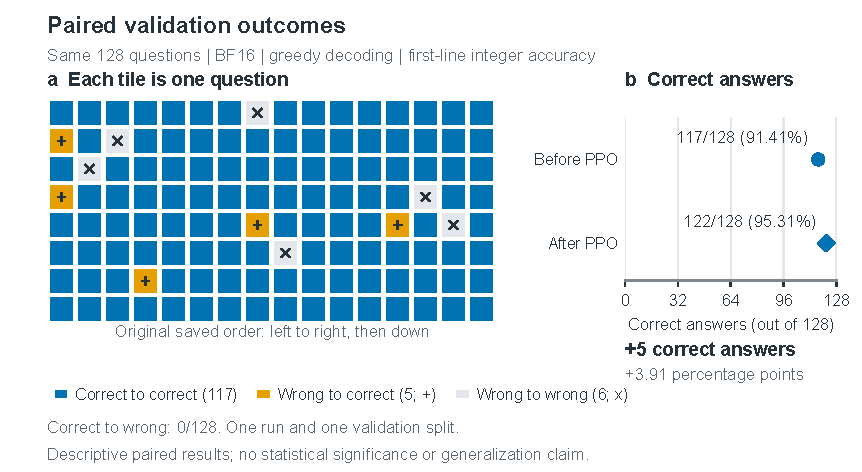
\includegraphics[width=146mm]{../../figures/paired_validation_outcomes.pdf}
\end{center}
\figcaption{fig:paired-zh}{保存题序中的 128 道题逐题配对。左图每格一题：117 题均正确、5 题由错变对、6 题均错误；右图给出正确数和正确率。每个状态均由原始回答重新评分，没有新增题目、重排以增强效果或添加统计显著性结论。}
\end{minipage}\par

\end{minipage}

\smallheading{保存与重载的实际范围}
Actor 已与基础模型一起在 GPU 上重新加载，通过有限值前向计算和生成检查。Critic 适配器通过哈希、有限值及非零更新检查，\key{没有独立重载 Critic}。保存的内容是 LoRA 适配器，不含基础模型权重，也不是可以完整恢复 PPO 优化器状态的检查点。原始回答、配置、标量指标和适配器保存在 \path{policy_adaptation/results/}。

\begin{minipage}{\linewidth}
\par\noindent\begin{minipage}{\linewidth}
\begin{center}
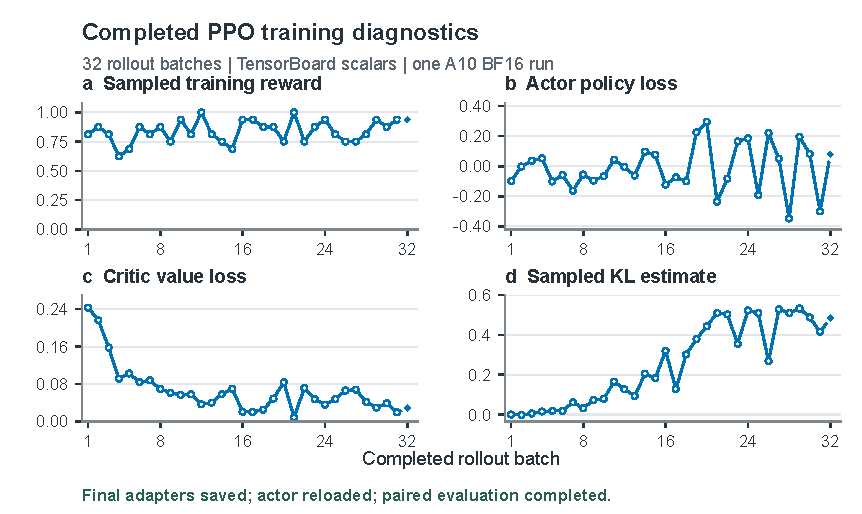
\includegraphics[width=146mm]{../../figures/ppo_training_success.pdf}
\end{center}
\figcaption{fig:ppo-curves-zh}{成功运行的四项训练诊断，每条曲线包含全部 32 个采样批次，每批 16 题。来自原始事件的数值未平滑，也未给单次运行添加置信区间。训练随机采样回答，温度为 1、top-$p$ 为 1；开发验证则使用贪心解码。}
\end{minipage}\par

\end{minipage}

平均任务奖励会随题目和采样回答波动，不能把首批与末批奖励之差解释成同条件正确率变化。Actor 策略损失可以为负，正负号不等于回答优劣；Critic 损失反映价值预测误差。记录的 KL 是采样估计，可能略小于零；理论 KL 散度本身仍非负。最后一批平均任务奖励为 0.9375，不能直接替代训练后验证正确率 0.953125。

\subsection{程序搜索的实际在线进展}
在线工程保存了 7 个方案记录：5 个完成有效评估，1 个因 Python 语法错误未能实现，另 1 个尚未评估。图表只统计实际完成且合法的结果，失败或缺失不会被填成零分。

\par\noindent\begin{minipage}{\linewidth}
\tablecaption{tab:online-scores-zh}{五次有效在线评估。时间均为 2026 年 10 月 31 日 UTC+08:00；第 0 代表示初始化。}
\begin{tabularx}{\linewidth}{@{}P{28mm}P{12mm}P{12mm}P{29mm}Y@{}}
\toprule
\tablehead \key{候选编号} & \key{代数} & \key{岛} & \key{分数} & \key{记录时间}\\
\midrule
\code{fe0aad416d4f} & 0 & 0 & 2.473873492 & 12:46:55\\
\code{4705b8e92e1b} & 0 & 1 & \key{2.620013807} & 13:08:21\\
\code{d3fb7a9f0bab} & 0 & 1 & 2.464972339 & 13:10:19\\
\code{34836c89e4f0} & 1 & 1 & 2.616027976 & 13:18:13\\
\code{a15ea29f0ceb} & 1 & 0 & 2.514353475 & 13:18:47\\
\bottomrule
\end{tabularx}
\end{minipage}\par


\begin{minipage}{\linewidth}
\par\noindent\begin{minipage}{\linewidth}
\begin{center}
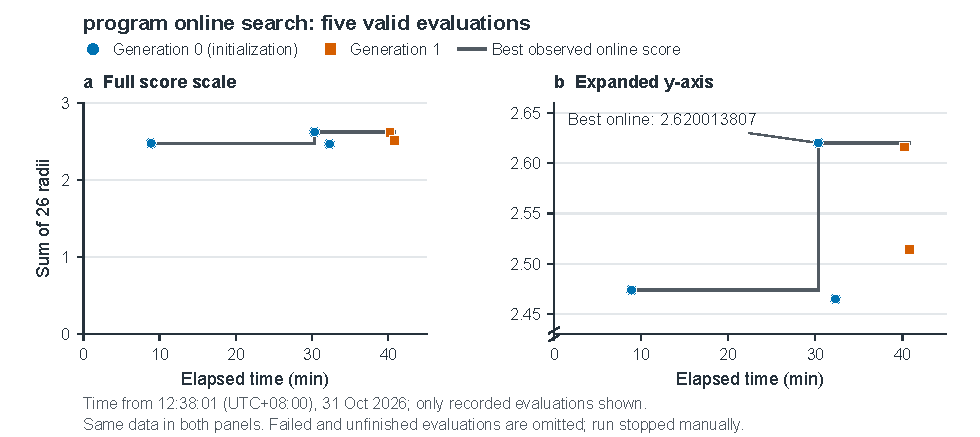
\includegraphics[width=166mm]{../../program_search/figures/online_progress.pdf}
\end{center}
\figcaption{fig:search-progress-zh}{同一组五次有效在线分数。左侧采用完整纵轴，右侧明确展示放大尺度；圆点为初始化，方点为第 1 代，阶梯线为累计最佳。没有推断第一条记录之前或最后一条之后的结果。}
\end{minipage}\par

\end{minipage}

累计最佳只对已经验证的集合定义：
\[
S_t^\star=\max_{a\in\mathcal V_t}S(a),\qquad \mathcal V_t\ne\varnothing.
\]
第一个分数为 2.473873492，之后一个初始候选达到完整精度的 2.62001380699489。第 1 代的坐标搜索子程序把自己的父程序从 2.473873492 提高到 2.514353475，但这一代的两个新程序都未超过全局最佳。结果证明流程能够生成、执行和筛选程序，不证明每代必然进步或找到了最优布局。

\subsection{最佳程序的独立复现}
导出的最佳候选 \code{4705b8e92e1b} 尝试 8 种固定初始布局，以 SLSQP 同时调整圆心和半径。圆心固定时，再求解
\[
\max_{\boldsymbol r}\ \sum_i r_i
\quad\text{满足}\quad
0\le r_i\le b_i,\quad r_i+r_j\le d_{ij},
\]
其中 $b_i=\min(x_i,y_i,1-x_i,1-y_i)$，$d_{ij}=\|\boldsymbol c_i-\boldsymbol c_j\|_2$。这是给定圆心下的线性规划；随后保守缩小半径以减轻浮点约束误差，不能由此证明圆心布局全局最优。

\begin{minipage}{\linewidth}
\begin{minipage}[c]{0.47\linewidth}
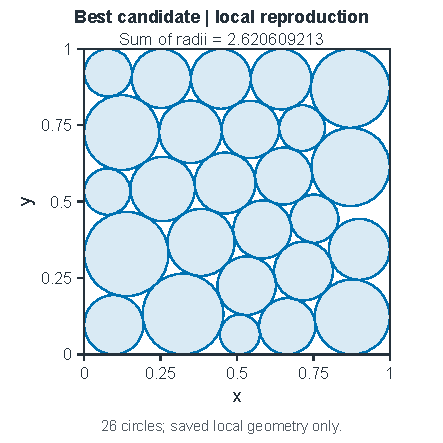
\includegraphics[width=75mm]{../../program_search/figures/online_best_reproduced.pdf}
\end{minipage}\hfill
\begin{minipage}[c]{0.49\linewidth}
\raggedright
未改动的导出程序在 Python 3.14.2、NumPy 2.4.4、SciPy 1.17.1 下约 4.76 秒完成本地复算。原几何方法接受全部 26 个圆；最小边界和圆间间隙约为 $1.38\times10^{-12}$ 与 $1.02\times10^{-12}$，均为正。

\key{在线记录：}2.62001380699489。\\
\key{本地复现：}2.6206092130170973。
\end{minipage}
\figcaption{fig:packing-zh}{最佳导出程序的本地复现布局。圆心、半径来自保存的几何数据，保持等比例，没有重新猜画位置。这不是服务器的原始坐标，也不是平台截图。}
\end{minipage}

两项分数约差 0.000595406。数值库或运行环境差异是一种可能解释，根因未证实。在线分数继续作为在线搜索结果，本地分数只支持独立复现记录；初始构造程序的本地值 0.959764 也不作为同一次在线实验的基线来计算百分比提升。

\section{讨论、局限与研究工程经历}
\subsection{反馈必须对应到实际评价目标}
两个案例都说明，过程中的反馈量与最终目标需要分别解释。PPO 的训练奖励来自不同题目和随机采样，任务变化应由同条件配对验证衡量；程序搜索中的漂亮解释或紧密图形，也必须经过原评估器执行后才算有效候选。本文保留生成失败、无效候选和缺失结果，避免只呈现成功记录。

参数优化案例回答了“能否走通并验证”的问题：完整训练、保存、Actor 重载和配对评估均已完成。程序搜索案例则展示了有限记录中的有效生成与选择，但全局最佳来自初始化，不能把“进行了演化”直接写成“每一代都带来提升”。两个任务的分数不可互相换算，也没有构成方法间公平竞赛。

\subsection{哪些限制仍然存在}
\begin{itemize}
\item \key{实验规模。}参数优化只使用一个种子、一个短算术任务和一个开发验证划分，没有多种子、独立测试集或消融比较。净增加五道正确题是描述性结果，不证明统计显著、最佳配置或通用推理能力提升。
\item \key{协议形成过程。}早期输出参与过首行答案规则的修订，因此不把当前验证集描述为从未查看的测试集。规则确定后的新 A10 前后比较保持一致，但不能消除整个开发过程的选择影响。
\item \key{保存范围。}Actor 实际重载已验证；Critic 只有适配器权重检查。其导出包含 LoRA 矩阵，却缺少底层随机初始化的价值头权重，因此仅凭这些文件无法重建完整的已训练价值函数。完整优化器恢复、长期续训和独立 Critic 重建未得到验证。
\item \key{搜索预算与终止。}圆装填仅五次有效评估，使用者在导出后手动停止。第 2 代开始不等于预算自动完成，也不能代表官方更大规模基准。
\item \key{可复现范围。}导出的代码和数据可复核，外部模型服务的生成响应不保证逐次相同。在线与本地数值差异的原因也未被单因素实验隔离。
\end{itemize}

\subsection{从失败恢复中形成的工程认识}
早期 T4 运行完成了 32 批计算，却在最终保存时因 PEFT 权重别名检查失败。这说明“训练循环结束”“模型成功保存”“重载后仍可使用”是不同证据。后续先做独立的 16 题保存重载检查，再进行完整运行，能够更早发现交付环节的问题；历史失败证据仍保留在附录~\ref{app:history-zh}，没有用新分数覆盖旧记录。

11 月 8 日的云端网络问题还阻碍了 FlashAttention 下载。源码检查确认当前单 GPU、未打包的 PPO 路径不会调用相关环形注意力功能，于是用哈希受约束的补丁延后三处导入。真正调用相关功能时仍需要真实依赖，没有实现假的算子。原依赖声明未篡改，\code{pip check} 中这一项缺失也被明确记录。此前的实际 CUDA Actor/Critic 前向反向检查和 FusedAdam 参数更新，随后完整运行，共同支持受限路径可用。

PPO 明确使用 eager 注意力；前后评估保留同一份原函数，可能使用 SDPA，没有强制改变实现。这里的工作是兼容性修复与运行验证，不是提出新的 PPO 算法，也没有把注意力实现选择当作性能改进的独立原因。

程序搜索早期有四次已完成的空代码回复，修正版提高输出上限并减少预算后才取得有效评估。思考耗尽输出额度是合理猜测，\cite{deepseek} 但同时改变了不止一个设置，也缺少完整结束原因，不能确认为单一根因。第 1 代日志报告的五次代码实现平均约 5 分 38 秒，评估平均约 30 秒；因此等待并不都来自几何计算。Planner 的 70,376 tokens 仅覆盖七个保存方案，不能冒充全任务成本。

\section{后续改进与可检验方案}
\subsection{以评估器证据约束反思和记忆}
重复的非法程序会浪费模型调用。可把重叠圆编号、越界、数组形状错误和超时整理为结构化反馈，附上相关代码，要求提出具体修复假设，再由原评估器验证。

平台已有错误反思和分层记忆。\cite{memory} 改进重点是更严格地筛选经验：每条经验关联候选、实测分数和评估器版本；区分已验证事实与猜测；移除重复、过期或矛盾内容；每次只检索少量相关记录。例如，经检查能够保持约束的半径更新值得保存，自称高分却越界的程序不能成为成功经验。

预期收益是减少重复错误、提高合法候选比例，但反思与检索会消耗 tokens，陈旧经验也可能把搜索带偏。验证时固定模型、评估器和总预算，比较不使用这类记忆与使用已验证记忆的运行；跨多个种子记录合法率、重复失败率、最佳有效分数和成本。本文没有执行这组对照实验。

\subsection{保留搜索多样性，并依据实际进展分配预算}
若每个提示都模仿当前最佳代码，搜索可能重复同一方向。可给不同岛分配不同提示角色：局部微调当前布局、探索新空间排列、优先生成可靠几何构造。各岛仍使用同一目标与评估器，完全重复的代码先去重，候选只定期交换。

分岛与迁移本来就是框架机制。\cite{islands} 进一步的研究问题是，能否依据有效分数、停滞和失败率分配后续调用：某方向长期无进展时，把部分预算留给替代方向。模型可以建议切换，但最终资源分配依据应是实际评估，而不是自然语言解释是否新颖。

多样性可能帮助离开局部最优，自适应分配也可能减少重复调用；代价是探索弱方向和短运行的不稳定。公平实验应固定总调用量或 token 成本，对比统一提示、固定分配与多角色提示、自适应分配；用多个种子报告最佳有效分数的中位数和分布、独特合法候选数及达到预设目标的耗时。这里仍是待验证方案，没有声称已经获得改进。

\smallheading{共同的评估边界}
评估器应位于模型不可修改的区域，候选程序最终独立复核，失败也应保留。对于单个 26 圆实例，结论只限该实例；改变问题规模或任务后仍需重新测试。两种提案都不必先重训大语言模型，却都需要真实对照结果才能成为有效方法的证据。

\section{结论}
本研究完成了低秩适配实现验证，以及Qwen 基座上的完整小规模 PPO 流程。在固定开发验证条件下，正确数由 117/128 变为 122/128；Actor 可保存并重载，Critic 适配器通过权重检查。第二个案例以真实在线调用生成并评估了五个合法圆装填候选，最佳在线分数为 2.62001380699489，独立本地复现记录另行保存。两项研究支持有限任务下的实现可行性与可检查结果，不提供普遍能力、全局最优或新算法的证明。

对后续研究而言，主要尚未回答的问题是不同种子、任务和预算下的稳定性，以及两项代理改进能否在相同成本下减少无效搜索。原始程序、回答、几何数据、失败记录和源码版本为这些进一步实验提供了起点。

\renewcommand{\refname}{参考文献}
\begin{thebibliography}{99}
\small
\setlength{\itemsep}{4pt}
\bibitem{lora}
E. J. Hu et al. \textit{LoRA: Low-Rank Adaptation of Large Language Models}. 2021.
\href{https://arxiv.org/abs/2106.09685}{arXiv:2106.09685}.
\bibitem{lorasurvey}
Y. Mao et al. \textit{A Survey on LoRA of Large Language Models}. 2024.
\href{https://arxiv.org/abs/2407.11046}{arXiv:2407.11046}.
\bibitem{lorablog}
J. Schulman et al. \textit{LoRA Without Regret}. Thinking Machines Lab, 29 September 2025.
\href{https://thinkingmachines.ai/blog/lora/}{Empirical analysis of LoRA fine-tuning}.
\bibitem{qwen}
Qwen Team. \href{https://huggingface.co/Qwen/Qwen2.5-0.5B}{Qwen2.5-0.5B model card};
\href{https://modelscope.cn/models/Qwen/Qwen2.5-0.5B}{official ModelScope repository}.
Pinned Hugging Face revision: \code{060db6499f32faf8b98477b0a26969ef7d8b9987}.
\bibitem{ppo}
J. Schulman, F. Wolski, P. Dhariwal, A. Radford and O. Klimov.
\textit{Proximal Policy Optimization Algorithms}. 2017.
\href{https://arxiv.org/abs/1707.06347}{arXiv:1707.06347}.
\bibitem{openrlhf}
OpenRLHF Team. OpenRLHF v0.6.0, commit \code{bfa85f6fa8cd6214707f93883fac5d08334f4f06}.
\href{https://github.com/OpenRLHF/OpenRLHF/blob/bfa85f6fa8cd6214707f93883fac5d08334f4f06/openrlhf/cli/train_ppo.py}{Training entry point};
\href{https://github.com/OpenRLHF/OpenRLHF/blob/bfa85f6fa8cd6214707f93883fac5d08334f4f06/openrlhf/models/actor.py}{Actor};
\href{https://github.com/OpenRLHF/OpenRLHF/blob/bfa85f6fa8cd6214707f93883fac5d08334f4f06/openrlhf/models/model.py}{Critic};
\href{https://github.com/OpenRLHF/OpenRLHF/blob/bfa85f6fa8cd6214707f93883fac5d08334f4f06/openrlhf/trainer/ppo_utils/experience_maker.py}{sampling and advantage estimation};
\href{https://github.com/OpenRLHF/OpenRLHF/blob/bfa85f6fa8cd6214707f93883fac5d08334f4f06/openrlhf/utils/deepspeed/deepspeed.py}{saving logic}.
\bibitem{torch}
PyTorch Team. PyTorch v2.5.1.
\href{https://github.com/pytorch/pytorch/blob/v2.5.1/torch/cuda/__init__.py}{CUDA BF16 capability detection and the \code{including\_emulation} argument}.
\bibitem{llm4ad}
Optima-CityU. \href{https://github.com/Optima-CityU/LLM4AD_Next/tree/dfde353e753e9021fffe88b5b034bf0c84d90b60}{LLM4AD\_Next / OpenLoopX};
\href{https://llm4ad-next.cn/}{hosted service}.
Source-study commit: \code{dfde353e753e9021fffe88b5b034bf0c84d90b60}.
\bibitem{architecture}
LLM4AD\_Next. \href{https://github.com/Optima-CityU/LLM4AD_Next/blob/dfde353e753e9021fffe88b5b034bf0c84d90b60/docs/en/architecture/overview.md}{Architecture Overview}.
Pinned source revision as above.
\bibitem{dataflow}
LLM4AD\_Next. \href{https://github.com/Optima-CityU/LLM4AD_Next/blob/dfde353e753e9021fffe88b5b034bf0c84d90b60/docs/en/architecture/data-flow.md}{Data Flow}.
Initialization, evolution, state and export boundaries.
\bibitem{islands}
LLM4AD\_Next. \href{https://github.com/Optima-CityU/LLM4AD_Next/blob/dfde353e753e9021fffe88b5b034bf0c84d90b60/docs/en/guides/island-ga.md}{Island GA guide}.
\bibitem{memory}
LLM4AD\_Next. \href{https://github.com/Optima-CityU/LLM4AD_Next/blob/dfde353e753e9021fffe88b5b034bf0c84d90b60/docs/en/guides/memory.md}{Long-term Memory guide}.
\bibitem{benchmark}
LLM4AD\_Next. \href{https://github.com/Optima-CityU/LLM4AD_Next/blob/dfde353e753e9021fffe88b5b034bf0c84d90b60/examples/applications/alphaevolve_math_benchmark/README.md}{AlphaEvolve Mathematics Benchmark Suite}.
Task definitions, objective directions and published-score provenance.
\bibitem{circle}
LLM4AD\_Next circle-packing example:
\href{https://github.com/Optima-CityU/LLM4AD_Next/blob/dfde353e753e9021fffe88b5b034bf0c84d90b60/examples/applications/alphaevolve_math_benchmark/circle_packing/code_config.yaml}{configuration};
\href{https://github.com/Optima-CityU/LLM4AD_Next/blob/dfde353e753e9021fffe88b5b034bf0c84d90b60/examples/applications/alphaevolve_math_benchmark/circle_packing/algorithm/solve.py}{initial constructor};
\href{https://github.com/Optima-CityU/LLM4AD_Next/blob/dfde353e753e9021fffe88b5b034bf0c84d90b60/examples/applications/alphaevolve_math_benchmark/circle_packing/evaluator.py}{geometry evaluator}.
\bibitem{deepseek}
DeepSeek. \href{https://api-docs.deepseek.com/guides/thinking_mode/}{Thinking Mode};
\href{https://api-docs.deepseek.com/api/create-chat-completion/}{Chat Completions API}.
\end{thebibliography}


\clearpage
\appendix
\section{手工适配器实现与检查}\label{app:implementation-zh}
\path{policy_adaptation/lora_training.py} 的核心职责包括：验证输入；共享并冻结原权重；为 $A$ 使用 Kaiming-uniform 初始化、为 $B$ 使用全零初始化；实现低秩修正分支；在推理时合并权重并避免重复合并；递归替换目标线性层；统计总参数和可训练参数。

对 24 层 Qwen 模型的 CPU/float32 功能检查替换了 168 个投影层。基础模型参数为 494,032,768，新增适配器参数为 4,399,104，占合并统计总数的 0.8826\%。该检查完成前向计算和权重合并，其入口没有完整的语言模型优化循环，因此不能由它单独推断训练效果。该功能配置的 dropout 为 0.05；正式 PPO 配置为 0。

九项轻量测试分别覆盖初始等价、共享权重、非零修正公式、合并等价与幂等性、冻结基座后的优化器更新、嵌套替换和参数统计、非法输入、数据划分及只针对回答评分的本地 HTTP 接口。测试中的小型线性层实际执行了优化器更新；这与完整语言模型 PPO 实验是不同层级的证据。

\section{在线搜索记录与停止范围}\label{app:online-zh}\label{app:source-zh}
修订配置于 2026 年 10 月 31 日 12:38:01 启动。最后保存的事件时间为 13:21:18.838，工程于 13:22:05 导出，随后手动停止。以上时间均为 UTC+08:00。没有自动完成事件，不能声称完整配置预算已自动执行。

更早一次尝试保留了五个方案，但没有有效评估，其中四次已完成的代码回复为空。修订同时提高输出上限（4,096 到 32,768）并缩小搜索预算，不能把恢复归因于单一参数。保存的 Planner 记录累计 70,376 tokens，只覆盖相应记录，不代表全部任务成本。公开证据保留候选程序、配置和五次有效分数，省略包含账号界面的截图；实际在线最佳布局的原始坐标未导出，报告中的最佳布局来自独立本地执行。

源码分析固定 LLM4AD\_Next 提交为 \code{dfde353e753e9021fffe88b5b034bf0c84d90b60}，不保证托管网站与该提交完全一致。在线模型由平台报告为 \code{deepseek-v4-flash}，本文没有独立验证服务内部模型实现。

\section{历史保存失败和成功恢复}\label{app:history-zh}
早期 FP32 T4 运行完成了 512 题、32 个采样批次，但在最终保存时出现共享权重别名检查错误：
\begin{Verbatim}[fontsize=\small,breaklines=true,frame=single]
AssertionError: mismatch keys {'base_model.model.lm_head.weight'}
RuntimeError: training failed (exit 1)
\end{Verbatim}
该次运行的开发基准为 118/128，没有有效的最终适配器和训练后评估。它不能与 A10 的训练后结果配对。历史曲线来自原控制台的舍入数值，必须与 A10 的精确事件记录分别解释。

\begin{center}
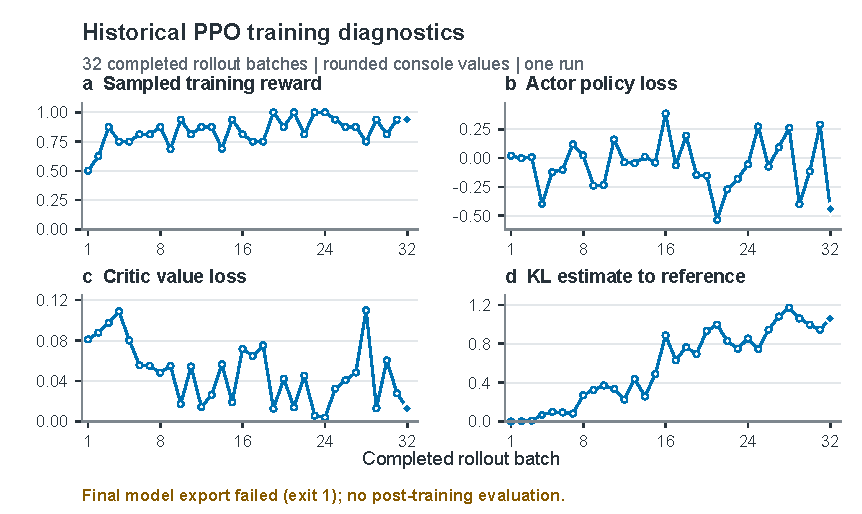
\includegraphics[width=146mm]{../../figures/observed_attempt.pdf}
\end{center}
\figcaption{fig:historical-zh}{早期 T4 的历史训练诊断。32 批计算完成后仍发生最终保存失败；曲线不能代替保存和重载证据，也不代表后来 A10 的结果。}

保存修复仅在输出层权重与输入嵌入是同一个 Parameter 时接受缺失的别名，真正缺少独立权重仍会报错。另一个采样器修复补齐 \code{pad\_len=None}。最终采用单 GPU eager attention 路径，关闭 packing 和 ring attention，并对固定源码做哈希检查后延迟三个未使用的 ring 操作导入。它不模拟 FlashAttention 的计算，若调用真实 ring 操作仍要求安装该依赖。

环境元数据保留了一项已声明的例外：OpenRLHF 0.6.0 要求 FlashAttention，但它未安装。真实 CUDA Actor/Critic 前向、反向和 FusedAdam 参数更新通过后，又通过独立 16 题的保存及 Actor 重载检查，再从原始基座开始完整运行。成功环境为 Python 3.10、PyTorch 2.5.1+cu124、Transformers 4.48.3、PEFT 0.14.0、DeepSpeed 0.16.3、Ray 2.42.0。PPO 显式使用 eager；原评估函数可能使用 SDPA。

成功运行于 2026 年 11 月 8 日 09:48:14 UTC 完成。约九秒后另一调用因已有受保护产物而被拒绝，其导出清单因而记录后一次调用失败。它不推翻前一次的退出码 0、完整 32 批指标、有限且非零的适配器、Actor 实际重载和逐题回答。原始本地导出单独保留；公开版本仅整理便携证据子集。Critic 只检查了权重，没有独立重载，也没有完整的 PPO 优化器恢复检查点。

\section{复现材料的阅读顺序}\label{app:reproduction-zh}
先阅读 \path{policy_adaptation/results/} 中训练前后的逐题回答和采样指标，再对照训练配置、适配器检查和模型修订。历史 T4 保存失败的指标必须单独阅读。\path{program_search/} 中的在线评估 CSV 与本地保存坐标是两种记录，不能互相替代。

\path{policy_adaptation/} 提供手工 LoRA、固定参数训练入口、奖励服务、共同评估函数和兼容修复；\path{program_search/} 提供最佳导出构造程序和几何检查。公开副本只规范身份信息和特定机器路径，不改变实验数值或适配器权重。绘图入口读取保存数据，不发起训练或在线搜索；本地重新执行构造程序则会产生新的本地计算记录，数值可能随库版本变化。

全新环境安装脚本是整理后的复现方案，尚未在另一台干净 GPU 机器上重复完整实验。免费 GPU、网络与外部模型服务可用性仍是外部条件。依赖安装、基础检查和显式训练命令见仓库中英文说明；轻量检查不等于重新完成 PPO 或托管搜索。

\end{document}
